\cleardoublepage
\chapter{Theoretical Framework}
\label{sec:dev}

\section{Endrov}
\label{sec:endrov}



\section{Thresholding}
\label{sec:thresholding}

Thresholding is a process of image segmentation that can be used to create
binary images from grayscale images.A binary image is a type of discrete image in
 which the value of a pixel is either $1$ or $0$ depending on whether the pixel belongs
to the foreground or to the background.

As stated on \cite{web:thresholding} during the thresholding process, individual 
pixels in an image are marked as ``object'' pixels if 
their value is greater than some threshold value (assuming an object to be brighter than the 
background) and as ``background'' pixels otherwise. This convention is known as \emph{threshold above}. 
Variants include \emph{threshold below}, which is opposite of threshold above; \emph{threshold inside}, where a 
pixel is labeled "object" if its value is between two thresholds; and \emph{threshold outside}, which is 
the opposite of \emph{threshold inside} \cite{shapiro}. Typically, an object pixel is given 
a value of $0$ while a background pixel is given a value of $1$ Finally, a binary image is 
created by coloring each pixel white or black, depending on a pixel's label.\\

In image processing applications where the study is focused on particular objects contained
in an image, thresholding becomes an effective and simple tool to separate these objects from
the background. Commongly, the gray levels belonging to the object are substantially
different from the gray levels of the background pixels. In \cite[p.146]{thres} many thresholding
applications on image processing are mentioned such as: document image analysis, where the goal
is to extract printed characters, logos, graphical content, or musical scores; map processing
where lines, legends and characters are to be found; scene processing, where a target is to
be detected; and quality inspection of materials, where defective parts must be delineated,
among many others. \\

The key parameter in the thresholding process is the thresholding value (or values for
\emph{threshold inside approach}). The value can be automatically computed, what is called
\emph{automatic thresholding}, as well as set or tuned through user input.\\
According to the information they are exploiting, the different thresholding methods can be 
categorized. In \cite[p.147]{thres}, Sezgin and Sankur categorize the thresholding methods in
six groups:
\begin{itemize}
\item Histogram shape-based methods: the peaks, valleys and curvatures of the smoothed
histogram are analyzed
\item Clustering-based methods: gray-level samples are clustered in two parts as
background and foreground, or modeled as a mixture of two Gaussians.
\item Entropy-based methods: algorithms that use the entropy of the foreground 
and background regions, the cross-entropy between the original and binarized image, 
etc.
\item Object attribute-based methods:Ssearch a measure of similarity between the 
gray-level and the binarized images, such as fuzzy shape similarity, 
edge coincidence, etc.
\item Spatial methods: use higher-order probability distribution and/or 
correlation between pixels
\item Local methods: adapt the threshold value on each pixel
to the local image characteristics.
\end{itemize}

Below, in Fig.\ref{fig:thres1}, two images are shown that correspond to a grayscale image
and binary image obtained by thresholding.

\begin{figure}
  \centering
  \subfloat[Grayscale Image]{\label{fig:threso}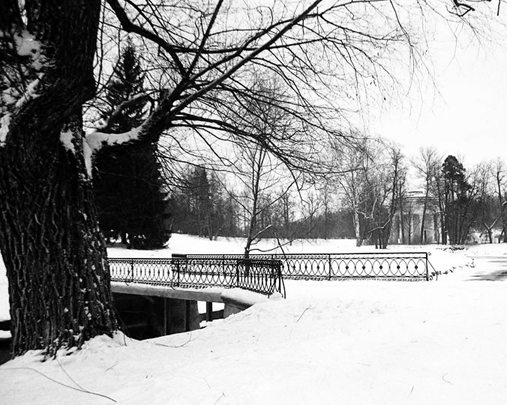
\includegraphics[width=0.45\textwidth]{thres/winter_o}}
\qquad
  \subfloat[After Threshold effect image]{\label{fig:thres1}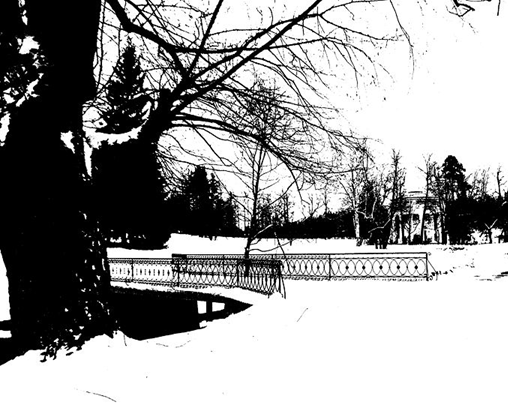
\includegraphics[width=0.45\textwidth]{thres/winter_thres}}
  \caption{Grayscale Image before and after a thresholding effect is applied. Images taken from \cite{web:thresholding}}
  \label{fig:thres1}
\end{figure}

\section{Distance Transform}
\label{sec:dt}

A distance transform or distance map is a representation of a digital image
that is obtained by converting a digital binary image, consisting in object
and non-object pixels, to another image in which each pixel has a value
corresponding to the distance to the nearest non-object pixel. The object 
pixels can be considered as foreground and the non-object pixels as
background. The obtained image is then a sort of grayscale representation
of the foreground pixels in the binary image.\\
The pixel mapping depends mainly on the distance metric, which is the 
measurement method of distance between image pixels. Different metrics have been 
studied  to find distance maps such as 
\emph{City Block or Manhattan},
\emph{Chessboard}, \emph{Euclidean}, \emph{Chamfer 3-4}, \emph{Octogonal}, among
others.\cite[p.363]{dtresearch}. There exist a great amount of
distance metric of other kinds, that are useful for different purposes.
These are commongly derived from the previous.
Below are shown the images obtained by applying different distance metrics.

\begin{figure}[h t b p ! H]
 \centering
   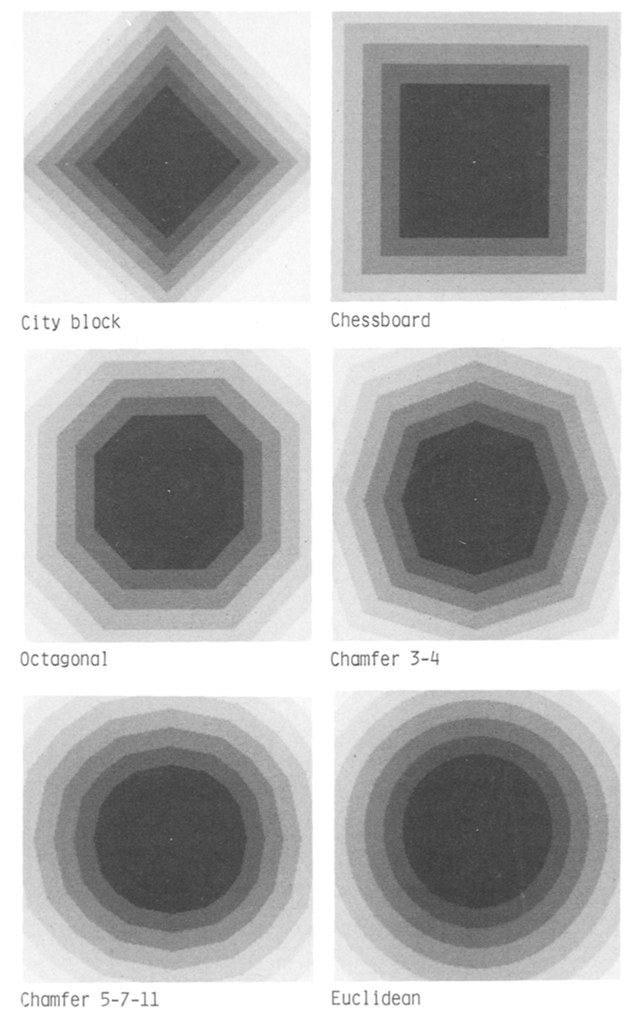
\includegraphics[scale=0.4]{dt/dtref}
 \caption{The distances from a point for the six DTs.
 The lighter the color the larger the distance \cite[p.365]{dtresearch}}
\end{figure}

As stated on \cite{dtresearch2} 
Distance transforms play a central role in the comparison of binary images, 
particularly for images resulting from local feature detection techniques such 
as edge or corner detection. For example, both the Chamfer
and Hausdorff matching approaches make use of distance transforms in comparing binary images. 
Distance maps can also be interpreted as landscapes of islands 
where the label of every pixel indicates the height of the region. This allows
the detection of ridges and peaks which is a straightforward way to find the
skeleton of an object.\cite[237]{ridgedt}. The nature of distance transforms
in which the objects are represented as contour layers of different depth
makes them also a useful tool to edge analysis and to improve efficiency of 
morphology algorithms such as \emph{Thinning} and \emph{Thickening}.\\

\section{Skeletonization}
\label{sec:skeletonization}


\section{Image Segmentation}
\label{sec:segmentation}

\subsection{Clustering}
\label{sec:clustering}

\section{Shape Matching}
\label{sec:shapefitting}

Shape matching is a central problem in visual information systems,
computer vision, pattern recognition, and robotics \cite{matchingbook}.It consist in identifying the area or contour of an specifical
 shape or class of shapes in an image, and plays a fundamental
role in content extraction from images and content-based image
retrieval. In \cite{matching2} Veltkamp explains that shape 
matching deals with transforming a shape and measuring the 
resemblance with another one, using some similarity measure, that 
normally correspond to the notion of distance between shapes.\\
The concept of shape is abstract, but most approaches in 
shape matching represent a shape as a geometrical object.
This can be both a set of points, curves, surfaces, solids,etc.
and a geometrical pattern modulo some transformation group,
in particular similarity transformations (translations, rotations 
and scalings), as it is stated on \cite{matching2}.\\

There are different studied ways to approach the shape matching 
problem. Since the approach followed in this thesis work
is related to those that deal with computational geometry, the
emphasis on this section will be on the last ones. Computational
Geometry studies algorithms that can be declared in terms of 
geometry.\\

In \cite{matchingbook} Veltkamp and Hagedoorn mention different 
approaches of shape matching such as: tree prunning, the
generalized Hough transform or pose clustering, geometric hashing,
the alignment method, statistics, deformable templates, relaxation
labeling, Fourier descriptors, wavelet transform, curvature
scale space and neural networks.
They also categorize the matching techniques in two main groups:
\emph{global image transforms} and \emph{global objects methods}.
The \emph{global image transform} group refers to the techniques that
``transform the image from color information in the spatial
domain to color variation in the frequency domain''. 
These approaches do not represent the shape explicitly for 
matching, instead they represent color or intensity transitions 
in the image. This makes impossible to measure the difference of 
two images in terms of shape as well as match a shape with a 
specifical part of an image.\\
On the other hand the \emph{global object methods} work with a complete
object area or contour and can analyze specifical areas in the 
image instead of requiring to process the whole image as in 
the global image transforms. In order to perform a proper
matching, the objects in the image have to be completely and
clearly segmented. Some of these methods are: \emph{moments}, where an
object is described as a set of moments, \emph{modal matching},
where the boundary is used insted of the area and is described 
with Fourier descriptors and \emph{curvature scale space}, where a a
scale space and parameterized representation of the contour of the 
objects is used.\\

Veltkamp describes in \cite{matching2} four different forms in
which shape matching is studied, given two shape patterns
and a dissimilarity measure. These are:

\begin{itemize}
\item \textbf{Computation Problem: }Compute the dissimilarity
  between the two patterns
\item \textbf{Decision Problem: }For a given threshold, decide
  whether the dissimilarity is smaller than the threshold
\item \textbf{Decision Problem: }For a given threshold, decide
  whether there exists a transformation such that the
dissimilarity between the transformed pattern and the other 
pattern is smaller than the threshold
\item \textbf{Optimization Problem: }Find the transformation
that minimizes the dissimilarity between the transformed
pattern and the other pattern.
\end{itemize}

A well studied optimization approach for shape matching is
Active Contour Models (\emph{Snakes}), in which is inspired much 
of the shape fitting approach of this work 
(see Sec \ref{sec:metfit}).In \cite{snakes} a snake is defined 
as an energy-minimizing spline guided by external constraint
forces and influenced by image forces that pull it toward 
features such as lines and edges. The \emph{snakes} are said to
be active contour models because they lock onto nearby edges,
localizing them accurately.\\
The \emph{snakes} model is defined as a controlled continuity spline that is bound
to internal and external image forces, called energies. The external energy models how well
the deformed model matches the data. The internal energy models
the objects resistance to be pushed by the external force into directions not coherent
with the prior knowledge, as it is stated on \cite{deformable}.The internal energy  imposes the 
a ``piecewise smoothness constraint'',\cite{snakes}. This means that a contour is
pushed to an image feature by the external force while the contour itself exhibits resistance
to be deformed into a non-smooth curve. \\

Given these definitions, let $M$ be the model and $D$ a data set
the energy $E$ can be defined as:

$$E(M) = E_{ext}(M,D) + E_{int}(M)$$

where $E_{ext}$ is the external energy function and $E_{int}$ the 
internal energy function.As it is explained on \cite{deformable} the image forces push the snake toward
salient image features like line, edges and subjective contours, while the external constraint forces
are responsible for putting the snake near the desired local minimun.
The optimization algorithm will consist then in minimizing this objective
function until the best solution is found.

\section{Cardinal Splines}
\label{sec:splines}

\section{Triangle mesh and rasterization}
\label{sec:triangle}


